%
%===============>>  ГРУППА 9-2 МОДУЛЬ 9 <<=============
%
\setmodule{9}

%BEGIN_FOLD % ====>>_____ Занятие 1 _____<<====
\begin{class}[number=1]
	\begin{listofex}
		\item Найдите значение выражения: \(\dfrac{ 9,4 }{ 4,1+5,3 }\).
		\item На координатной прямой отмечены числа \( a \) и \( b \). Какое из следующих утверждений неверно?
		\begin{center}
			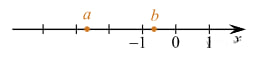
\includegraphics[align=t, width=0.5\linewidth]{\picpath/G93M8L6-6}
		\end{center}
		\begin{tasks}(2)
			\task \( a+b<0 \)
			\task \( -2<b-1<-1 \)
			\task \( a^2b<0 \)
			\task \( -a<0 \)
		\end{tasks}
		\item Найдите значение выражения \( \dfrac{a^{17}\cdot(b^5)^3}{(a\cdot b)^{15}} \) при \( a=7 \) и \( b=\sqrt{7} \).
		\item Решите уравнения: \(\dfrac{ 3 }{ x-19 }=\dfrac{ 19 }{ x-3 }\). \\
		Если корней несколько, запишите их в ответ без пробелов в порядке возрастания.
		\item В фирме такси в данный момент свободно \(15\) машин: \(3\) чёрных, \(6\) жёлтых и \(6\) зелёных. По вызову выехала одна из машин, случайно оказавшаяся ближе всего к заказчику. Найдите вероятность того, что к нему приедет жёлтое такси.
		\item На одном из рисунков изображен график функции \(y=x^2-2x+3\). Укажите номер этого рисунка.
		\begin{center}
			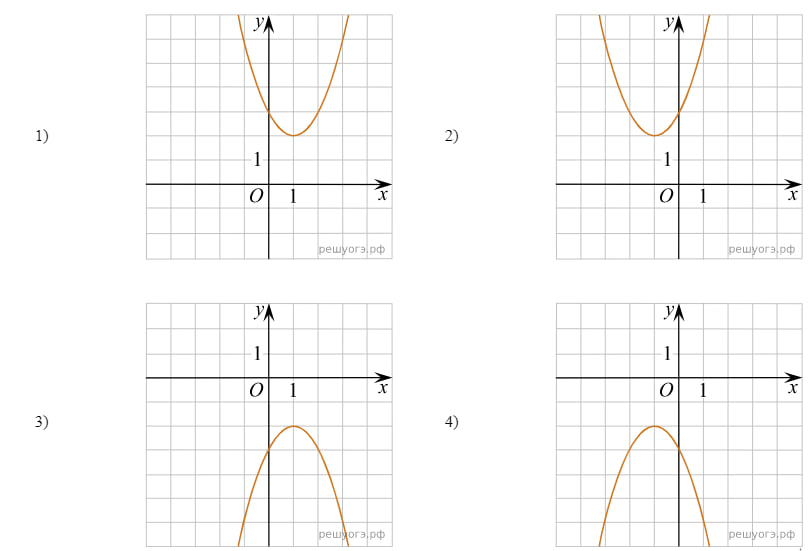
\includegraphics[align=t, width=0.9\linewidth]{\picpath/G91M9L1}
		\end{center}
		\item Объём пирамиды вычисляют по формуле \(V=\dfrac{ 1 }{ 3 }Sh\),  где \(S\) --- площадь основания пирамиды, \(h\) --- её высота. Объём пирамиды равен \(40\), площадь основания \(15\). Чему равна высота пирамиды?
		\item Решите неравенство: \(-x^2-2x\le0\).
		\item В амфитеатре \(14\) рядов. В первом ряду \(20\) мест, а в каждом следующем на \(3\) места больше, чем в предыдущем. Сколько мест в десятом ряду амфитеатра?
		\item В равностороннем треугольнике \(ABC\) биссектрисы \(CN\) и \(AM\) пересекаются в точке \(P\). Найдите \(\angle MPN\).
		\item К окружности с центром в точке \(O\) проведены касательная \(AB\) и секущая \(AO\). Найдите радиус окружности, если \(AB=12\) см, \(AO=13\) см.
		\item В треугольнике одна из сторон равна \(10\), другая равна \(10\sqrt{3}\), а угол между ними равен \(60\degree\). Найдите площадь треугольника.
		\item Основания трапеции равны \(18\) и \(12\), одна из боковых сторон равна \(4\sqrt{2}\), а угол между ней и одним из оснований равен \(135\degree\). Найдите площадь трапеции.
		\item Укажите номера верных утверждений.
		\begin{tasks}
			\task Если три угла одного треугольника равны трем углам другого треугольника, то такие треугольники подобны. 
			\task Сумма смежных углов равна \(180\degree\).
			\task Любая медиана равнобедренного треугольника является его биссектрисой.
		\end{tasks}
		\item Решите уравнение: \(x^2-2x+\sqrt{3-x}=\sqrt{3-x}+8\)
		\item Из пункта \(A\) в пункт \(B\), расстояние между которыми \(13\) км, вышел пешеход. Одновременно с ним из \(B\) в \(A\) выехал велосипедист. Велосипедист ехал со скоростью, на \(11\) км/ч большей скорости пешехода, и сделал в пути получасовую остановку. Найдите скорость пешехода, если известно, что они встретились в \(8\) км от пункта \(B\).
		\item Постройте график функции \(y=\dfrac{ (x+1)(x^2+7x+12) }{ x+3 }\) и определите, при каких значениях \(m\) прямая \(y=m\) имеет с графиком ровно одну общую точку.
		\item Периметр прямоугольника равен \(30\), а диагональ равна \(14\). Найдите площадь этого прямоугольника.
		\item Докажите, что медиана треугольника делит его на два треугольника, площади которых равны между собой.
		\item Основание \( AC \) равнобедренного треугольника \( ABC \) равно \( 12 \). Окружность радиуса \( 8 \) с центром вне этого треугольника касается продолжений боковых сторон треугольника и касается основания \( AC \) в его середине. Найдите радиус окружности, вписанной в треугольник \( ABC \).
	\end{listofex}
\end{class}
%END_FOLD

%BEGIN_FOLD % ====>>_____ Занятие 2 _____<<====
\begin{class}[number=2]
	\begin{listofex}
		\item Занятие 2
	\end{listofex}
\end{class}
%END_FOLD

%BEGIN_FOLD % ====>>_ Домашняя работа 1 _<<====
\begin{homework}[number=1]
	\begin{listofex}
		\item Домашняя работа 1
	\end{listofex}
\end{homework}
%END_FOLD

%BEGIN_FOLD % ====>>_____ Занятие 3 _____<<====
\begin{class}[number=3]
	\begin{listofex}
		\item Занятие 3 
	\end{listofex}
\end{class}
%END_FOLD

%BEGIN_FOLD % ====>>_____ Занятие 4 _____<<====
\begin{class}[number=4]
	\begin{listofex}
		\item Занятие 4
	\end{listofex}
\end{class}
%END_FOLD

%BEGIN_FOLD % ====>>_ Домашняя работа 2 _<<====
\begin{homework}[number=2]
	\begin{listofex}
		\item Решите систему уравнений: \( \begin{cases} x-y=-5; \\ x^2-2xy-y^2=17 \end{cases} \)
		\item Игорь и Паша красят забор за \( 8 \) часов. Паша и Володя красят этот же забор за \( 9 \) часов, а Володя и Игорь --- за \( 24 \) часа. За сколько минут мальчики покрасят забор, работая втроём?
		\item Постройте график функции \( y=|x+1|-|x-1|-x \) и найдите все значения \( k \), при которых прямая \( y=kx \) имеет с графиком данной функции ровно одну общую точку.
		\item Расстояние от точки пересечения диагоналей ромба до одной из его сторон равно \( 14 \), а одна из диагоналей ромба равна \( 56 \). Найдите углы ромба.
		\item 
		\begin{minipage}[t]{\bodywidth}
			Два равносторонних треугольника имеют общую вершину. Докажите, что отмеченные на рисунке отрезки \( AB \) и \( CD \) равны.
		\end{minipage}
		\gapwidth
		\begin{minipage}[t]{\picwidth}
			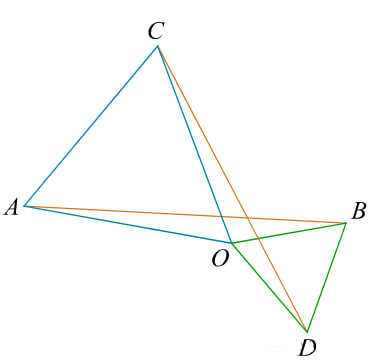
\includegraphics[align=t, width=\linewidth]{\picpath/G91M9H2}
		\end{minipage}
	\end{listofex}
\end{homework}
%END_FOLD

%BEGIN_FOLD % ====>>_____ Занятие 5 _____<<====
\begin{class}[number=5]
	\begin{listofex}
		\item Занятие 5
	\end{listofex}
\end{class}
%END_FOLD

%BEGIN_FOLD % ====>>_____ Занятие 6 _____<<====
\begin{class}[number=6]
	\begin{listofex}
		\item Занятие 6
	\end{listofex}
\end{class}
%END_FOLD

%BEGIN_FOLD % ====>>_ Домашняя работа 3 _<<====
\begin{homework}[number=3]
	\begin{listofex}
		\item Домашняя работа 3
	\end{listofex}
\end{homework}
%END_FOLD

%BEGIN_FOLD % ====>>_____ Занятие 7 _____<<====
\begin{class}[number=7]
	\title{Подготовка к проверочной}
	\begin{listofex}
		\item Занятие 7
	\end{listofex}
\end{class}
%END_FOLD

=%BEGIN_FOLD % ====>>_ Проверочная работа _<<====
\begin{exam}
	\begin{listofex}
		\item Проверочная
	\end{listofex}
\end{exam}
%END_FOLD